\section{Asservissement par méthodes de Reinforcement Learning}

En intelligence artificielle, plus précisément en apprentissage automatique, l'apprentissage par renforcement consiste, pour un agent autonome (robot, etc.), à apprendre les actions à effectuer à partir d'expériences, de façon à optimiser une récompense quantitative au cours du temps. L'agent est plongé au sein d'un environnement, et prend ses décisions en fonction de son état courant. En retour, l'environnement procure à l'agent une récompense, qui peut être positive ou négative. L'agent cherche au travers d'expériences itérées un comportement décisionnel optimal, appelé stratégie ou politique, et qui est une fonction associant à l'état courant l'action à exécuter. Son but étant de trouver le meilleur comportement décisionnel maximisant la somme des récompenses au cours du temps.

Nous allons plus précisément parler ici de Deep Reinforcement Learning, puisqu’il s’agit de la fusion de deux mondes qui sont l’apprentissage par renforcement qui émerge de la programmation dynamique, et du Deep Learning.

\begin{figure}[H]
    \centering
    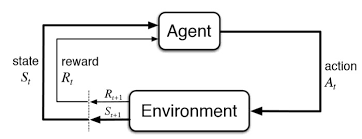
\includegraphics[width=0.5\textwidth]{./image_RL/image30.png}
    \caption{Schéma reinforcement learning}
\end{figure}

\subsection{Reinforcement}

Avant même de comprendre l’intérêt du Deep Learning dans les méthodes de renforcement, il faut comprendre le fonctionnement de cette méthode d’apprentissage. En effet, le Q-Learning ou reinforcement est plus ancien et donc utilisé depuis plus longtemps que le Deep Learning en programmation dynamique. Le principe du Q-Learning est  d’estimer la qualité de l’action ou de l’état d’un agent dans un environnement donné. Pour estimer cette qualité, on fait appelle aux processus de décision markoviens qui sont synthétisés par l’équation de Bellman

\begin{figure}[H]
    \centering
    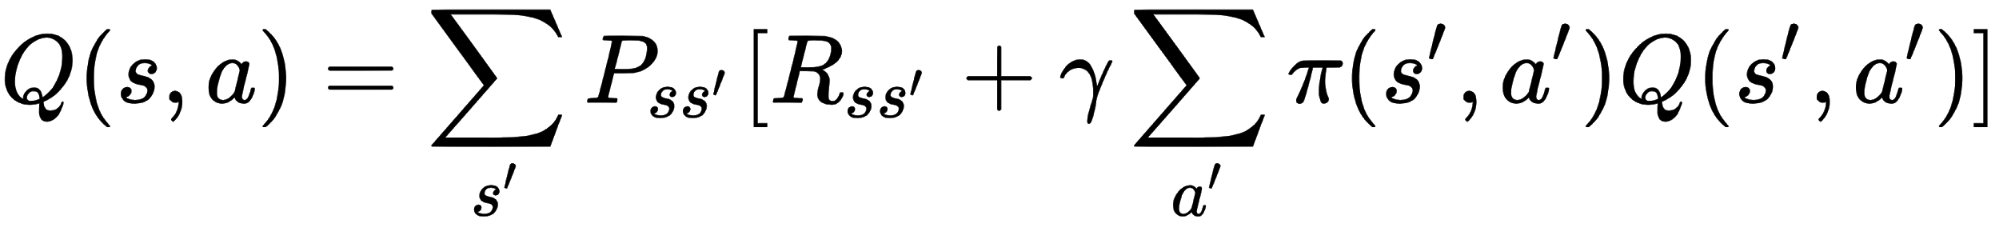
\includegraphics[width=0.5\textwidth]{./image_RL/image22.png}
    \caption{Equation de Bellman}
\end{figure}

Dans cette équation, S représente l’état de l’agent à un instant t et S’ celle de l’agent à l’instant t+1. Comme on peut le constater, cette équation est récursive, elle permet de quantifier la qualité d'une action ou d'un état à l'instant t grâce à celle définie à l'instant t+1.
Ainsi l'agent perçoit son environnement grâce à ces transitions que l'on appelle le MDP (Markovian decision process)

Au début du renforcement, cette méthode était utilisée pour des environnements discrets et pas trop volumineux. En effet, si on considère que l’agent évolue dans un damier de 3x3 il n’y a que 9 états possibles et donc on peut facilement mettre à jours les valeurs d’un état ou d’une action en utilisant la programmation dynamique.
Mais cette méthode est très limité lorsqu’on parle d’un environnement avec plus de $10^{6}$ états possible par exemple.
C’est là qu'intervient le Deep Learning.

\subsection{Deep Reinforcement Learning}

En programmation dynamique, il faut absolument stocker les valeurs des différentes qualités des états dans une matrice ou autre, ce qui n’est pas le cas dans les méthodes de deep reinforcement learning.
En effet, les réseaux de neurones sont des estimateurs universels. On les utilise aussi bien en classification d’image que pour des problèmes d’estimations de prix d’une maison.
Ainsi, plutôt que de stocker la valeur d’un état ou d’une action, nous pouvons la ré-estimer à chaque instant.

\subsection{Méthodes d'apprentissages}

En reinforcement, l’objectif est d'entraîner le réseau de neurones pour qu’il trouve une politique (un comportement) optimal par rapport à l’environnement.
Pour ce faire, il faut définir au préalable une fonction de reward. En effet, à chaque instant le robot va évoluer avec son environnement et recevoir une récompense. 
Les méthodes développées visent à optimiser la policy ( politique de l’agent) de façon à maximiser ces récompenses.

